\let\negmedspace\undefined
\let\negthickspace\undefined
\documentclass[journal]{IEEEtran}
\usepackage[a5paper, margin=10mm, onecolumn]{geometry}
%\usepackage{lmodern} % Ensure lmodern is loaded for pdflatex
\usepackage{tfrupee} % Include tfrupee package

\setlength{\headheight}{1cm} % Set the height of the header box
\setlength{\headsep}{0mm}     % Set the distance between the header box and the top of the text

\usepackage{gvv-book}
\usepackage{gvv}
\usepackage{cite}
\usepackage{amsmath,amssymb,amsfonts,amsthm}
\usepackage{algorithmic}
\usepackage{graphicx}
\usepackage{textcomp}
\usepackage{xcolor}
\usepackage{txfonts}
\usepackage{listings}
\usepackage{enumitem}
\usepackage{mathtools}
\usepackage{gensymb}
\usepackage{comment}
\usepackage[breaklinks=true]{hyperref}
\usepackage{tkz-euclide} 
\usepackage{listings}
% \usepackage{gvv}                                        
\def\inputGnumericTable{}                                 
\usepackage[latin1]{inputenc}                                
\usepackage{color}                                            
\usepackage{array}                                            
\usepackage{longtable}                                       
\usepackage{calc}                                             
\usepackage{multirow}                                         
\usepackage{hhline}                                           
\usepackage{ifthen}                                           
\usepackage{lscape}
\usepackage{circuitikz}
\begin{document}

\bibliographystyle{IEEEtran}
\vspace{3cm}

\title{}
\author{EE24BTECH11053 - S A Aravind Eswar
}
% \maketitle
% \newpage
% \bigskip
{\let\newpage\relax\maketitle}

\renewcommand{\thefigure}{\theenumi}
\renewcommand{\thetable}{\theenumi}
\setlength{\intextsep}{10pt} % Space between text and floats


\numberwithin{equation}{enumi}
\numberwithin{figure}{enumi}
\renewcommand{\thetable}{\theenumi}

\begin{enumerate}
    \item Read the two statements related to sintering and select the correct option.\\

    Statement-1: Sintering in vacuum leads to improved densification as compared to sintering under ambient (at atmospheric pressure) condition.\\

    Statement-2: Closed pores formed during sintering inhibit full densification.\hfill{[2020 - XE]}
    \begin{enumerate}
        \item Both Statement-1 and Statement-2 are FALSE
        \item Both Statement-1 and Statement-2 are TRUE
        \item Statement-1 is TRUE but Statement-2 is FALSE
        \item Statement-1 is FALSE but Statement-2 is TRUE
    \end{enumerate}

    \item Select the correct option that appropriately matches the process to the material/product that can be fabricated using them. \hfill{[2020 - XE]}
    \begin{table}[h]
        \centering
        \begin{tabular}{|m{5em} | m{5em} | m{10em} |}
	\hline
	\textbf{Symbol} & \textbf{Value} &\textbf{Description}\\
	\hline
		\textbf{A} & $\myvec{0\\0}$ & Point \textbf{A}\\
	\hline
		\textbf{B} & $\myvec{x\\-4}$ & Point \textbf{B}\\
	\hline
		$d$          & 5              & Distance between points \textbf{A} and \textbf{B}\\
	\hline
\end{tabular}

    \end{table}
    \begin{enumerate}
        \item I-S, II-P, III-R, IV-Q
        \item I-S, II-R, III-Q, IV-P
        \item I-S, II-P, III-Q, IV-R
        \item I-P, II-R, III-Q, IV-S
    \end{enumerate}
    \item Consider a FCC structured metal with lattice parameter a = 3.5 \r{A}. If the material is irradiated using X-rays of wavelength $\lambda$ = 1.54056 \r{A}, the Bragg angle (2$\theta$) corresponding to the fourth reflection will be: \hfill{[2020 - XE]}
    \begin{enumerate}
        \item 88.21$^\circ$
        \item 76.99$^\circ$
        \item 99.35$^\circ$
        \item 93.80$^\circ$
    \end{enumerate}
    
    \item The number of Schottky defects per mole of KCI at 300 $^\circ$C under equilibrium condition will be: \hfill{[2020 - XE]}
    
    Given:\\
    Activation energy for the formation of Schottky defect = 250 $kJ.mol^{-1}$\\
    Avogadro number =  $6.023 \times 10^23 mol^{-1}$\\
    Universal Gas Constant = $8.314 J.K^{-1}.mol^{-1}$
    \begin{enumerate}
        \item 1.21 x 10$^{18}$
        \item 1.52 x 10$^{16}$
        \item 9.75
        \item 2.42 x 10$^{12}$
    \end{enumerate}
    
    \item In an industry, the probability of an accident occurring in a given month is $\frac{1}{100}$ Let P(n) denote the probability that there will be no accident over a period of 'n' months. Assume that the events of individual months are independent of each other. The smallest integer value of 'n' such that P(n)$\leq \frac{1}{2}$ is \underline{\hspace{3cm}} (\textit{round off to nearest integer}) \hfill{[2020 - XE]}
    
    \item For a FCC metal, the ratio of surface energy of \{111\} surface to \{100\} surface is \underline{\hspace{3cm}} (round-off to two decimal places). Assume that only the nearest neighbor broken bonds contribute to the surface energy. \hfill{[2020 - XE]}
    \item  Pure silicon (Si) has a band gap (Eg) of 1.1 eV. This Si is doped with 1 ppm (parts per million) of phosphorus atoms. Si contains 5$\times 10^{28}$ atoms per m$^2$ in pure form. At temperature T = 300 K, the shift in Fermi energy upon doping with respect to intrinsic Fermi level of pure Si will be \underline{\hspace{3cm}} eV (\textit{with appropriate sign and round-off to two decimal places}).\\
    Intrinsic carrier concentration of Si, $n_i$, is given as:
    $$n_i = 2\brak{\frac{2\pi mk_B T}{h^2}}^{3/2} exp\brak{-\frac{E_g}{2k_B T}}$$
    Given:
    \begin{itemize}
        \item Mass of an electron, m = $9.1 \times 10^{-31} kg$
        \item Charge of an electron, e =$1.6 \times 10^{-19}$ C
        \item Boltzmann constant, $K_g = 1.38 \times 10^{-23} J.K^{-1}$
        \item Planck's constant, h = 6.6 $\times$ 10$^{-34}$ J.s
    \end{itemize}\hfill{[2020 - XE]}
    \item The schematic diagram shows the light of intensity Io incident on a material (shaded grey) of thickness, $x$, which has an absorption coefficient, $\alpha$ and reflectance, R. The intensity of transmitted light is I. The reflection of light (of a particular wavelength) occurs at both the surfaces (surfaces indicated in the diagram). The transmittance is estimated to be \underline{\hspace{3cm}} (\textit{round-off to three decimal places}).\\
    Given that for the wavelength used, $\alpha$ = 10$^3$ m$^{-1}$ and R = 0.05.\hfill{[2020 - XE]}
    % \resizebox{h-length}{v-length}{text}
\begin{figure}[h]
    \centering
    \resizebox{0.5\textwidth}{!}{%
    \begin{circuitikz}
    \tikzstyle{every node}=[font=\normalsize]
    \draw [line width=2pt, short] (0,17.5) -- (0,17.5);
    \draw [ fill={rgb,255:red,154; green,153; blue,150} , line width=0.2pt ] (0,18.75) rectangle (4.5,12.5);
    \draw [line width=2pt, short] (0,18.75) -- (0,12.5);
    \draw [line width=2pt, short] (4.5,18.75) -- (4.5,12.5);
    \draw [line width=2pt, <->, >=Stealth] (0,13.75) -- (4.5,13.75);
    \draw [line width=2pt, ->, >=Stealth] (-2.5,15) -- (0,15);
    \draw [line width=2pt, ->, >=Stealth] (5,15) -- (7.5,15);
    \node [font=\normalsize] at (-2.5,15.75) {$I_0$};
    \node [font=\normalsize] at (7,15.75) {$I$};
    \node [font=\normalsize] at (-1.75,14.5) {$Incident$};
    \node [font=\normalsize] at (-2,14) {$Light$};
    \node [font=\normalsize] at (6.25,14.5) {$Transmitted$};
    \node [font=\normalsize] at (6.5,14) {$Light$};
    \node [font=\normalsize] at (2,14.25) {$x = 3mm$};
    \node [font=\normalsize, rotate around={90:(0,0)}] at (0,11.25) {$Surface - 1$};
    \node [font=\normalsize, rotate around={90:(0,0)}] at (4.5,11.25) {$Surface - 2$};
    \end{circuitikz}
    }%
    
    \label{fig:my_label}
\end{figure}
    \item Fe$_3$O$_4$ (also represented as FeO.Fe$_2$O$_3$) is a FCC structured inverse spinel (AB$_2$O$_4$) material where 1/8 of tetrahedral sites are occupied by half of B cations and 1/2 of the octahedral sites are occupied by remaining B and A cations. The magnetic moments of cations on octahedral sites are antiparallel with respect to those on tetrahedral sites. Atomic number of Fe is 26 and that of O is 8. The saturation magnetic moment of Fe3O4 per formula unit in terms of Bohr magnetons ($\mu_B$) will be \underline{\hspace{3cm}} $\mu_B$. Ignore contribution from orbital magnetic moments. \hfill{[2020 - XE]}
    \item A piezoelectric ceramic with piezoelectric coefficient (d$_{zz}$) value of 100 x 10$^{-12}$ C.N$^{-1}$ is subjected to a force, $\vec{F_z}$, of 10 N, applied normal to its x-y face, as shown in the figure. If relative dielectric constant ($\epsilon_r$) of the material is 1100, the voltage developed along the z-direction of the sample will be Volts \underline{\hspace{3cm}}(\textit{round-off to two decimal places}). Ignore any nonlinear effects.\\
    Given: Permittivity of free space ($\epsilon_r$) is 8.85 x 10$^{-12}$ F.m$^{-1}$. \hfill{[2020 - XE]}
    \begin{tikzpicture}
    % Define dimensions
    \def\outerwidth{5}    % Outer square width (cm)
    \def\innerwidth{9.6}   % Inner square width (10 - 0.4, considering 0.2 cm gap on each side)
    \def\gap{0.2}          % Gap size (cm)
    \def\coilspacing{0.2}  % Coil spacing (cm)
    \def\coilloops{5}      % Number of coil loops

    % Outer square
    \draw[thick] (0,0) -- (6,0) -- (6,2.9) -- (5,2.9) -- (5,1) -- (1,1) -- (1, 5) -- (5, 5) -- (5,3.1) -- (6,3.1) -- (6, 6) -- (0, 6) -- (0,0);
    %\draw[thick] 
    \draw (0.5, 5.5) -- (0.5, 6.3);
    \draw (5.5, 5.5) -- (5.5, 6.3);
    \draw (.5, .5) -- (-.6, 0.5);
    \draw (.5, 5.5) -- (-.6, 5.5);
    % Inner square
    \draw[thick, dashed] (0.5, 0.5) rectangle (5.5,5.5);

    % Winding with current I
    \foreach \i in {1,...,\coilloops} {
        \draw[thick] (1, 4 - \i * \coilspacing - \coilspacing/2) to[out=180, in=0] 
            (0, 4 - \i * \coilspacing) ;
    }

    % Label the current I
    \node at (-.9, 3.35) {$I$};

    % Dimensions
    \draw[thick][->] (-0.2, 3.8) -- (0, 3.8);
    \draw[thick][<-] (-0.2, 2.9) -- (0, 2.9);
    \draw[<->] (0.5, 6.1) -- (5.5, 6.1) node[midway, above] {10 cm};
    \draw[<->] (-.5, 0.5) -- (-.5, 5.5) node[midway, left] {10 cm};
    \draw[<->] (6.2, 2.9) -- (6.2, 3.1) node[midway, right] {0.2 cm};
\end{tikzpicture}



    \item Silicon carbide (SiC) particles are added to Aluminum (Al) matrix to fabricate particle reinforced Al-SiC composite. The resulting composite is required to possess specific modulus (E/$\rho$; E: elastic modulus, p: density) three times that of pure Al. Assuming iso-strain condition, the volume fraction of SiC particles in the composite will be (\textit{round-off to two decimal places}). \hfill{[2020 - XE]}
    \begin{table}[h]
        \centering
        \begin{tabular}{| m{7em} | m{7em} | m{7em} |}
    \hline
    \textbf{Material} & \textbf{E(GPa)} & $\mathbf{\rho (g.cm^{-3})}$\\
    \hline
    \textbf{Al} & 69 & 2.70\\
    \hline
    \textbf{Si} & 379 & 2.36\\
    \hline
    
\end{tabular}
    \end{table}
    \item Isothermal weight gain per unit area ($\Delta$W/A, where $\Delta$W is the weight gain (in mg) and A is the area (in cm$^2$)) during oxidation of a metal at 600 $^\circ$C follows parabolic rate law, where, $\Delta$W/A = 1.0 mg.cm$^2$ after 100 min of oxidation. The $\Delta$W/A after 500 min at 600 $^\circ$C will be mg.cm$^2$ (round-off to two decimal places). \hfill{[2020 - XE]}
    \item A plain carbon steel sample containing 0.1 wt\% carbon is undergoing carburization at 1100 $^\circ$C in a carbon rich surroundings with fixed carbon content of 1.0 wt\% all the time. The carburization time necessary to achieve a carbon concentration of 0.46 wt\% at a depth of 5 mm at 1100 $^\circ$C is \underline{\hspace{3cm}}hour (round off to the nearest integer).\hfill{[2020 - XE]} \\
    Given: Diffusivity of carbon in iron at 1100 $^\circ$C is 6.0 $\times$ 10$^{-11}$ m$^2$.s$^{-1}$ and 
    \begin{table}[h]
        \centering
        \begin{tabular}{ m{3em} m{2em}}
    \hline
    \textbf{erf(z)} & \textbf{z}\\
    \hline
    0.56 & 0.55\\
    \hline
    0.60 & 0.60\\
    \hline
    0.64 & 0.65\\
    \hline
    0.68 & 0.70\\
    \hline

\end{tabular}
    \end{table}
\end{enumerate}

\end{document}  

